\documentclass{beamer}      % This is a beamer
\usepackage[utf8]{inputenc} % Language support
\usepackage{utopia}         % Utopia Font

\usetheme{Madrid}
\usecolortheme{default}

%------------------------------------------------------------
%Title configuration block
\title[Operating Systems]
{Operating Systems}

\subtitle{Beamer version 0.2}

\author[Fabricio Bortoluzzi]
{Fabricio Bortoluzzi\inst{1}}

\institute[UNIVALI]
{
  \inst{1}
  Computer Networks Laboratory\\
  in collaboration with\\
  Laboratory of Embedded and Distributed Systems\\
}

\date[UNIVALI 2019]
{www.univali.br\\leds.acad.univali.br}

%\logo{
\includegraphics[height=1.5cm]{images/univali-logo.jpg}}

%End of title configuration block
%------------------------------------------------------------

%------------------------------------------------------------
%The next block of commands puts the table of contents at the 
%beginning of each section and highlights the current section:

\AtBeginSection[]
{
  \begin{frame}
    \frametitle{Table of Contents}
    \tableofcontents[currentsection]
  \end{frame}
}
%------------------------------------------------------------

\begin{document}
%Create the title page.
\frame{\titlepage}

%---------------------------------------------------------
%This block of code is for the table of contents after
%the title page
\begin{frame}
\frametitle{Table of Contents}
\tableofcontents
\end{frame}
%---------------------------------------------------------

\section{Introduction}

%---------------------------------------------------------
\begin{frame}
    \frametitle{Hardware review}
    
    \begin{itemize}
        \item 
        A modern  computer  consists  of  one  or  more
        processors, some main  memory, disks,  printers,  
        a  keyboard,  a  mouse, a  display,  
        network  interfaces,  and  various other 
        input/output devices.

        \item 
        All in all, a complex system.
        
        \item 
        If every application programmer had to understand
        how all these things work in detail,
        no code would ever get written.

    \end{itemize}    

\end{frame}
%---------------------------------------------------------

%---------------------------------------------------------
\begin{frame}
    \frametitle{Wider definition of an Operating Systems}
    
    The operating system (OS) is a layer inserted 
    between the hardware/software interface in order
    to provide a 
    \begin{itemize}
        \item better
        \item simpler
        \item cleaner
    \end{itemize} 
    model of the computer.

\end{frame}
%---------------------------------------------------------

%---------------------------------------------------------
\begin{frame}
    \frametitle{Hardware support}
    
    Hardware must give proper support for protection.
    Minimal requirements are
    \begin{itemize}
        \item Processor Modes: Kernel and User
        \item MMU: Memory Management Unit
        \item I/O handling via interrupts
    \end{itemize}

\end{frame}
%---------------------------------------------------------

%---------------------------------------------------------
\begin{frame}
    \frametitle{Hardware support: Processor Modes}
    
    Processor Modes
    \begin{figure}
        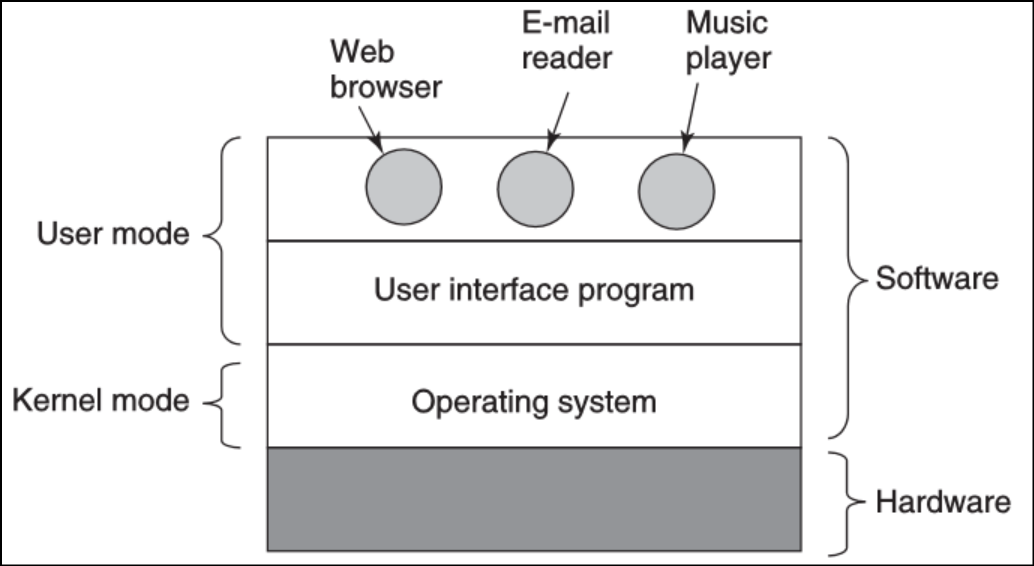
\includegraphics[scale=0.5]{images/101.png}
        \caption{The problem!}
    \end{figure}
    Continuing to processor mode

\end{frame}
%---------------------------------------------------------

%---------------------------------------------------------
\begin{frame}
    \frametitle{Hardware support: MMU}
    
    MMU: Memory Management Unit
    %\inputminted[c]{code/001.c}
    
\end{frame}
%---------------------------------------------------------

%---------------------------------------------------------
\begin{frame}
    \frametitle{Hardware support: I/O Interrupts}
    
    I/O Interrupts
    
\end{frame}
%---------------------------------------------------------

%---------------------------------------------------------
\begin{frame}
    \frametitle{The shell is not the OS}
    
    Users interact with the shell, either via 
    \begin{itemize}
        \item a Text Console; and/or
        \item the GUI - Graphical User Interface.
    \end{itemize}

\end{frame}
%---------------------------------------------------------


% INTRODUCTION QUIZ

%---------------------------------------------------------
\begin{frame}
    \frametitle{Quiz}
    
    \begin{itemize}
        \item
        1. What are the two main functions of an operating system?
        \item
        3. What is the difference between timesharing and multiprogramming systems?
        \item
        5. On early computers, e very byte of data read or written w as handled by the CPU (i.e.,
        there was no DMA). What implications does this have for multiprogramming?
    \end{itemize}    

\end{frame}
%---------------------------------------------------------

%---------------------------------------------------------
\begin{frame}
    \frametitle{Quiz}

        \begin{itemize}
        \item
        6. Instructions related to accessing I/O de vices are typically pri vileged instructions, that
        is, they can be executed in kernel mode but not in user mode. Give a reason why these
        instructions are privileged.
        \item 
        10. What is the difference between kernel and user mode? Explain how having two distinct
        modes aids in designing an operating system.
        \item 
        12. Which of the following instructions should be allowed only in kernel mode?
        (a) Disable all interrupts.
        (b) Read the time-of-day clock.
        (c) Set the time-of-day clock.
        (d) Change the memory map.
    \end{itemize}    

\end{frame}
%---------------------------------------------------------

%---------------------------------------------------------
\begin{frame}
    \frametitle{Quiz}
    
    \begin{itemize}
        \item 
        17. What is a trap instruction? Explain its use in operating systems.
        \item 
        25. What is the essential dif ference between a block special f ile and a character special
        file?
        \item
        27. Modern operating systems decouple a process address space from the machine’s physi-
        cal memory. List two advantages of this design.
    \end{itemize}    

\end{frame}
%---------------------------------------------------------  

%---------------------------------------------------------
\begin{frame}
    \frametitle{Quiz}
    
    \begin{itemize}
        \item
        29. Figure 1-23 sho ws that a number of UNIX system calls ha ve no Win32 API equi v-
        alents. For each of the calls listed as ha ving no Win32 equivalent, what are the conse-
        quences for a programmer of converting a UNIX program to run under Windows?
        \item
        30. A portable operating system is one that can be ported from one system architecture to
        another without any modification. Explain why it is infeasible to build an operating
        system that is completely portable. Describe two high-level layers that you will have in
        designing an operating system that is highly portable.
    \end{itemize}    

\end{frame}
%---------------------------------------------------------
\section{Memory Management}

%---------------------------------------------------------
%Basic frame
\begin{frame}
    \frametitle{First Frame of Memory Management}
    
    Text of the first frame of memory management.

\end{frame}
%---------------------------------------------------------

\section{File Systems}

%---------------------------------------------------------
%Basic frame
\begin{frame}
    \frametitle{First Frame of File Systems}
    
    Text of the first frame of file systems.

\end{frame}
%---------------------------------------------------------

\section{Input/Output}

%---------------------------------------------------------
%Basic frame
\begin{frame}
    \frametitle{First Frame of I/O}
    
    Text of the first frame of I/O.

\end{frame}
%---------------------------------------------------------

\section{Deadlocks}

%---------------------------------------------------------
%Basic frame
\begin{frame}
    \frametitle{Deadlocks}
    
    Text of the first frame of Deadlocks.

\end{frame}
%---------------------------------------------------------


%\section{Examples}

%---------------------------------------------------------
%Changing visivility of the text
\begin{frame}
    \frametitle{Sample frame title}
    This is a text in second frame. For the sake of showing an example.
    
    \begin{itemize}
        \item<1-> Text visible on slide 1
        \item<2-> Text visible on slide 2
        \item<3> Text visible on slides 3
        \item<4-> Text visible on slide 4
    \end{itemize}
    \end{frame}
    
    %---------------------------------------------------------
    
    
    %---------------------------------------------------------
    %Example of the \pause command
    \begin{frame}
    In this slide \pause
    
    the text will be partially visible \pause
    
    And finally everything will be there
    \end{frame}
    %---------------------------------------------------------
    
    \section{Processes and Threads}
    
    %---------------------------------------------------------
    %Highlighting text
    \begin{frame}
    \frametitle{Sample frame title}
    
    In this slide, some important text will be
    \alert{highlighted} because it's important.
    Please, don't abuse it.
    
    \begin{block}{Remark}
    Sample text
    \end{block}
    
    \begin{alertblock}{Important theorem}
    Sample text in red box
    \end{alertblock}
    
    \begin{examples}
    Sample text in green box. The title of the block is ``Examples".
    \end{examples}
    \end{frame}
    %---------------------------------------------------------
    
    
    %---------------------------------------------------------
    %Two columns
    \begin{frame}
    \frametitle{Two-column slide}
    
    \begin{columns}
    
    \column{0.5\textwidth}
    This is a text in first column.
    $$E=mc^2$$
    \begin{itemize}
    \item First item
    \item Second item
    \end{itemize}
    
    \column{0.5\textwidth}
    This text will be in the second column
    and on a second tought this is a nice looking
    layout in some cases.
    \end{columns}
    \end{frame}
    %---------------------------------------------------------
    
    

\end{document}